\glsresetall

\section{Bottlenecks in large scale microbial studies: sequence clustering}\label{section_bottlenecks}

Section~\ref{section_book} described in-depth a microbial community analysis pipeline.
In that pipeline, one of the most time consuming steps is performing
sequence clustering (also known as \gls{otu} picking). As a reminder, sequence
clustering is the processing step during which sequences are grouped into \gls{otu}s
based on sequence similarity. The \gls{otu}s found in a sample are used as an
approximation of the species richness in the given niche. Sequence similariy is
computed by sequence alignment \cite{Needleman1970, Smith1981}, an expensive
computation task that is quadratic based on the length of the input sequences. With
datasets containing from a few hundred thousand reads to a few billion
reads \cite{Goodwin2016}, performing all pairwise sequence alginments is too
computationally expensive to be performed in a timely manner. The sequence clustering
problem shares characteristics with the biological sequence database search problem,
which has been studied for more than 30 years. Sections~\ref{subsection_openref},
~\ref{subsection_soa} and~\ref{subsection_deblur}, contain a summary of my
contributions to optimize the sequence clustering step of microbial community
datasets analysis.

\subsection{Subsampled open-reference clustering creates consistent, comprehensive OTU definitions and scales to billions of sequences}\label{subsection_openref}

Section~\ref{section_book} described three different \gls{otu} picking approaches:
closed-reference, \emph{de-novo} and open-reference. The open-reference approach
was the recommended approach because it offers benefits over the other two
approaches. On one hand, the open-reference approach running time is shorter than
the \emph{de-novo} approach because it includes a parallel closed-reference step.
On the other hand, the open-reference approach doesn't discard any sequences from
the input dataset because it contains a \emph{de-novo} step. However, if the microbial
organisms present in an environment have not been previously characterized and included
in the reference database, a large portion of the sequences will fail to cluster
during the closed-reference step, generating long running times on the \emph{de-novo} step.
In order to further reduce the running time of the open-reference approach, we presented
a new approach: the subsampled open-reference approach \cite{Rideout2014}.

The following paragraphs have been adapted from the original publication in
\textsl{PeerJ, 2014}. As a contributor of this manuscript, I was involved on the
discussions for the design of the subsampled open-reference pipeline, contributed
to the source code, performed some of its evaluations, wrote sections of the
manuscript and reviewed drafts of the manuscript.

A detailed description of the workflow is illustrated in Figure~\ref{sub_open_ref_fig1}.
It is implemented using UCLUST v1.2.22q \cite{Edgar2010} for clustering in \gls{qiime} 1.6.0 \cite{Caporaso2010}
and later, though any sequence clustering software that provides support for \emph{de-novo}
and closed-reference clustering could be substituted for UCLUST in an alternate
implementation. The inputs provided to this method are demultiplexed,
quality-filtered sequences, and a reference sequence collection (for example,
the Greengenes 13 8 97\% \gls{otu} representative sequences \cite{DeSantis2006, McDonald2012}).
First, sequences are clustered in parallel using a closed-reference \gls{otu} picking
workflow, where sequences are queried against the reference database at percent
identity \emph{s} (default 97\%). If a read matches a reference sequence at greater
than or equal to \emph{s}\% identity, it is assigned to the \gls{otu} defined by that
reference sequence. These are referred to as the reference \gls{otu}s. Next, a
random subsample of \emph{n}\% (\emph{n} should be small, the default value in
\gls{qiime} 1.8.0-dev and earlier is 0.1\%) of the sequences that failed to match
the reference sequence collection are clustered \emph{de-novo}, and the cluster
centroids for all resulting \gls{otu}s are used to define a new reference sequence
collection. Those \gls{otu}s are referred to as the new reference \gls{otu}s.
The sequences that were not included in the random subsample that was clustered
\emph{de-novo} then go through an additional round of parallel closed-reference \gls{otu}
picking, this time where they are clustered against the new reference \gls{otu}s based
on matching a sequence in the new reference sequence collection at greater than
or equal to \emph{s}\% identity. This creation of a “new reference database”
allows us to harness the parallelization of our closed-reference \gls{otu} picking
pipeline, greatly decreasing the time it takes for sequences that fail to hit the
initial reference database to be clustered into \gls{otu}s. In the final clustering
step, sequences that fail to hit a reference sequence during this final
closed-reference \gls{otu} picking step are clustered \emph{de-novo}. These are
referred to as the clean-up \gls{otu}s. Finally, the reference \gls{otu}s, new
reference \gls{otu}s, and clean-up \gls{otu}s are combined into a single \gls{otu}
table (i.e., table of counts of \gls{otu}s on a per-sample basis, as described in
\cite{McDonald2012BIOM}), and this table, as well as a filtered table excluding
\gls{otu}s with counts less than or equal to a user-defined threshold \emph{c},
are provided to the user. By default, \emph{c = 2}, so each \gls{otu} is
observed at least twice (i.e., singleton \gls{otu}s are excluded). Because
many more of the sequences can be clustered using closed-reference \gls{otu}
picking in this workflow, it can run in far less time than classic
open-reference \gls{otu} picking.

\begin{figure}[htbp]
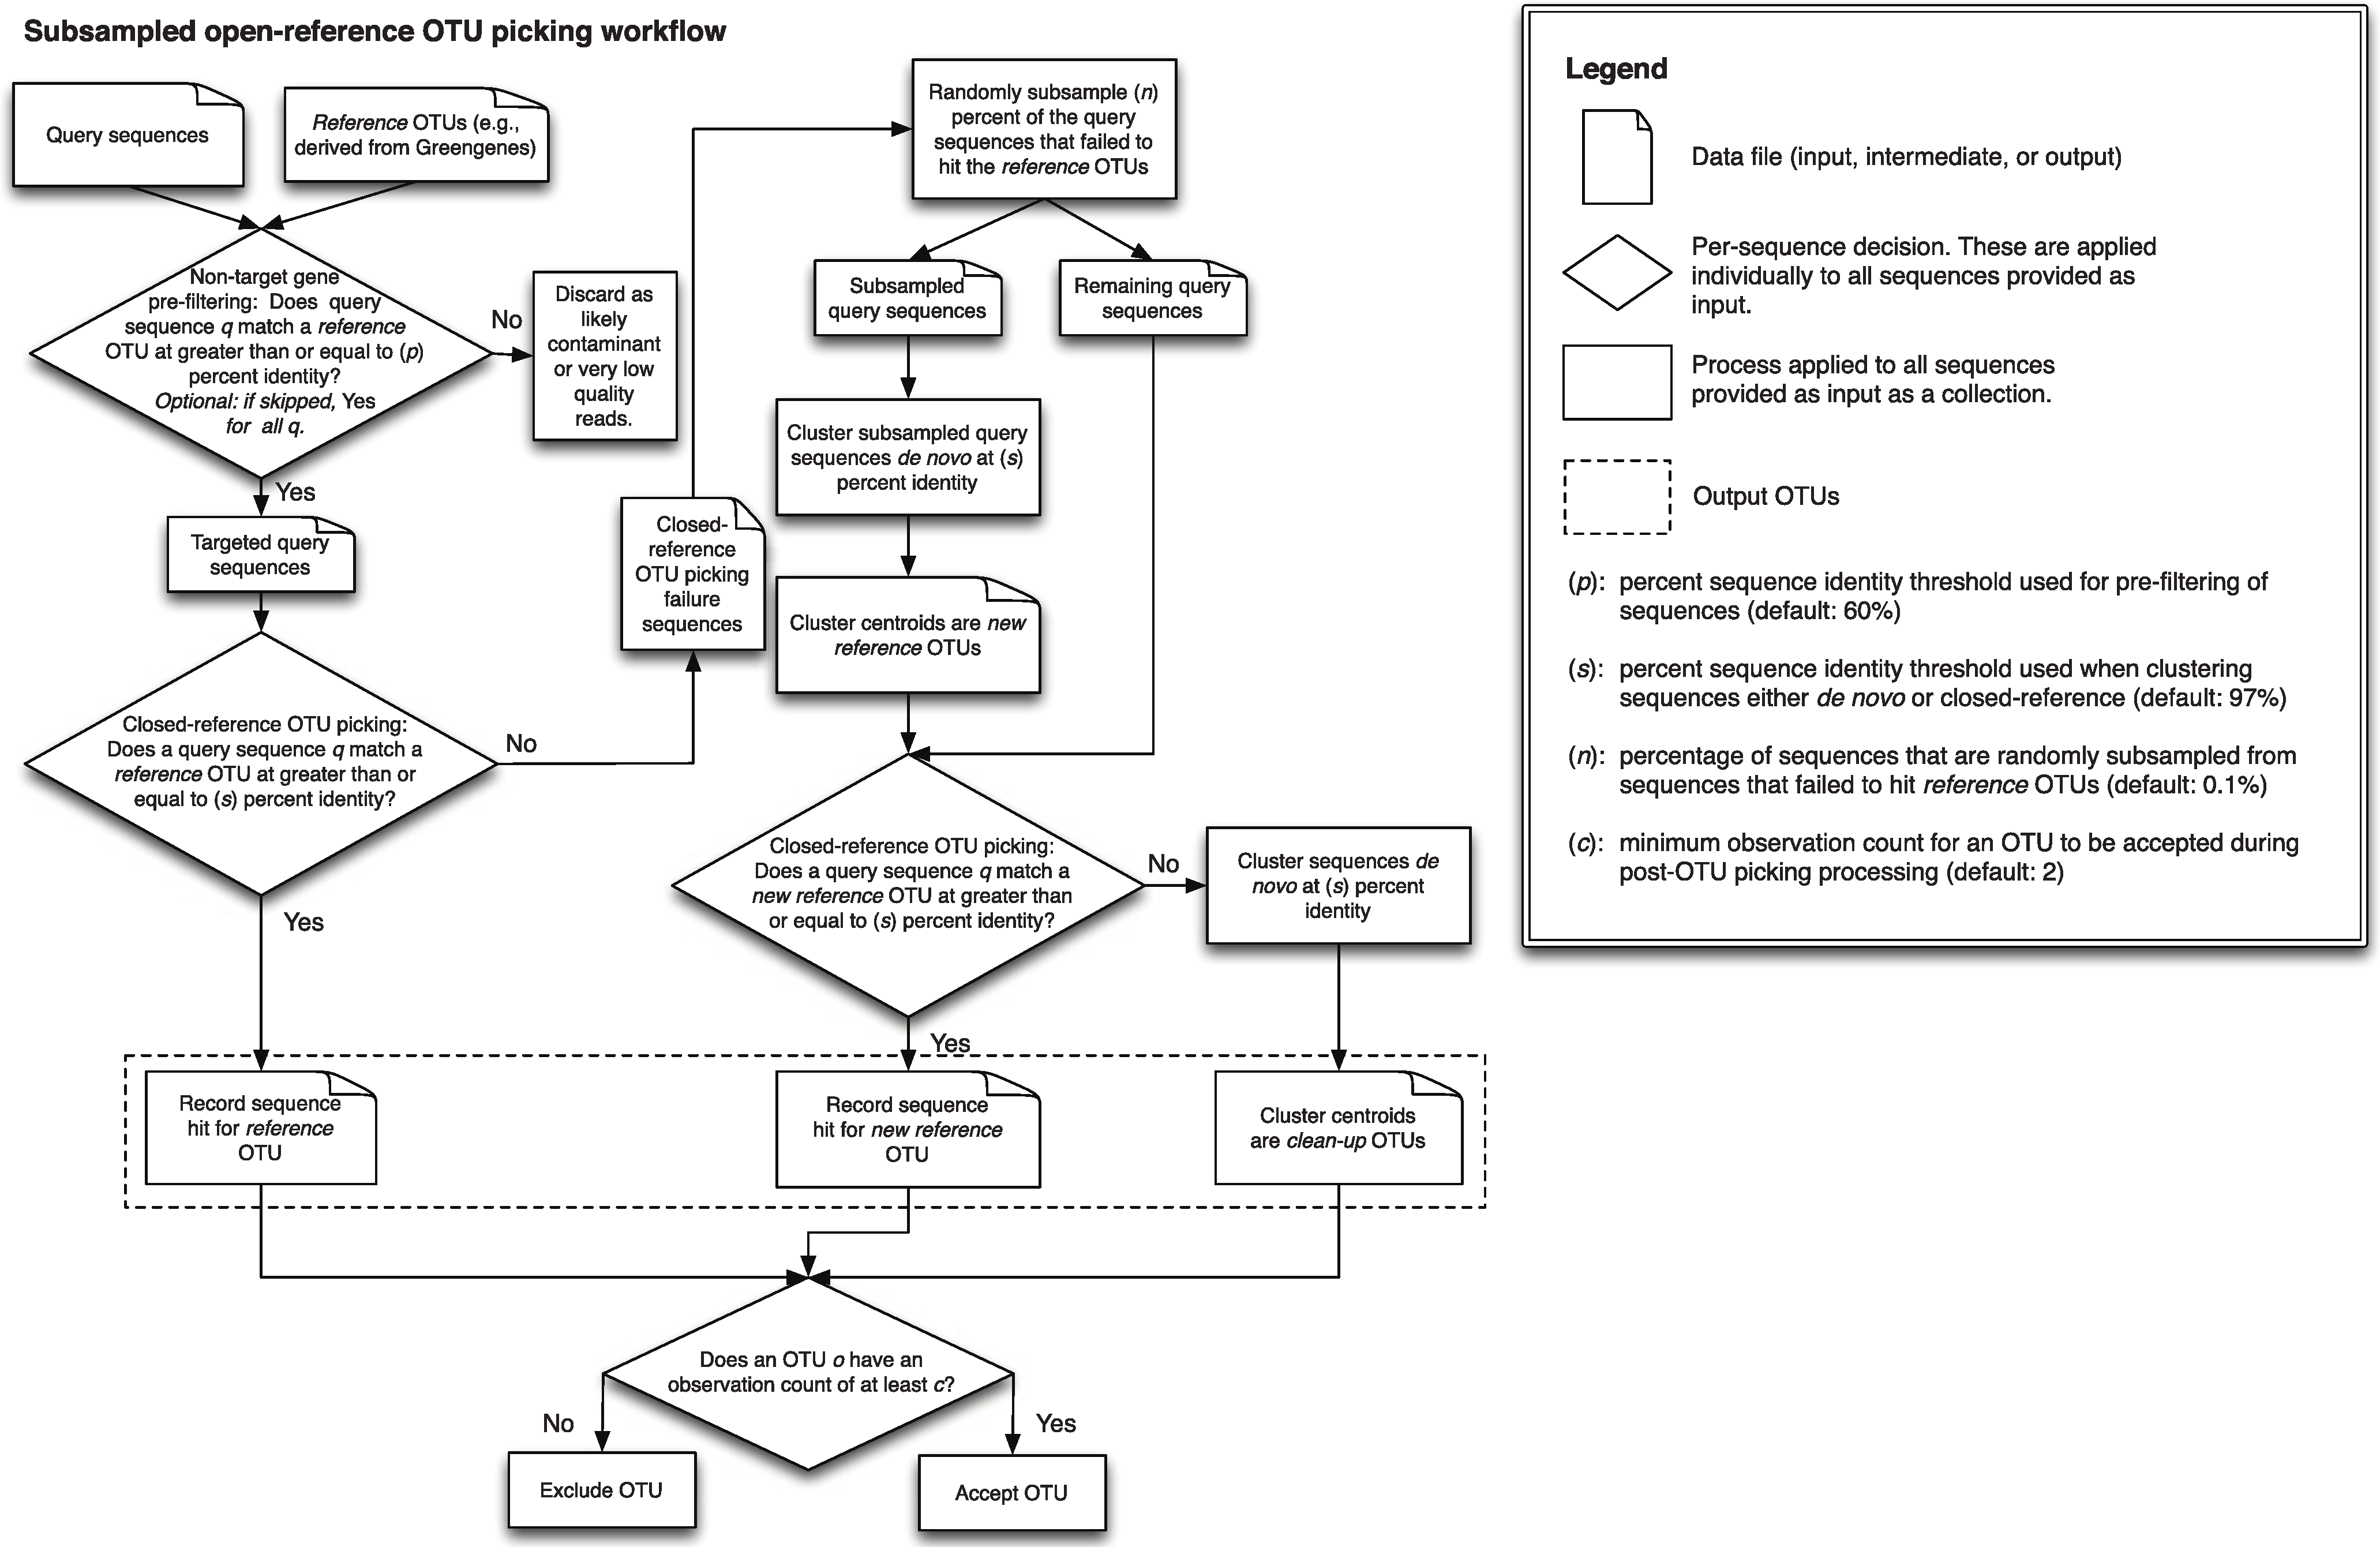
\includegraphics[width=\columnwidth]{chapter_otupicking_figures/workflow.png}
\caption[Schematic of the subsampled open-reference OTU picking algorithm]{\textbf{Schematic of the subsampled open-reference OTU picking algorithm.}}
\label{sub_open_ref_fig1}
\end{figure}

We validated the subsampled open-reference \gls{otu} picking workflow by comparing it
to the classic (i.e. non subsampled) open-reference clustering methods on three
different datasets: the Lauber "88 Soils" study \cite{Lauber2009} (referred to
as \emph{88-soils} here), the Caporaso "Moving Pictures" study \cite{Caporaso2011}
(referred to as \emph{moving-pictures} here), and the Costello "Whole Body" study
\cite{Costello2009} (referred to as \emph{whole-body} here) using three metrics.
First, we tested the correlation between sample alpha diversities (\gls{otu} counts,
i.e. \gls{qiime}'s \emph{observed species} metric and \gls{pd} \cite{Faith1992}) based
on subsampled open-reference \gls{otu} picking and the classic open-reference clustering.
Next, we tested whether beta diversity patterns (as determined by weighted and
unweighted UniFrac \cite{Lozupone2005} distances between samples) were consistent across \gls{otu}
picking protocols, based on Mantel tests \cite{Mantel1967} with 1,000 Monte Carlo iterations.
Finally we tested whether the same taxonomic profiles were obtained on a per-sample
basis using each of the \gls{otu} picking methods. It is important to note that
we are not trying to assess whether one method is better than another using these metrics.
Instead we are testing whether the methods give highly correlated results.

Alpha diversity (whole-body \gls{pd} Pearson \emph{r = 0.989}; 88-soils \gls{pd}
Pearson \emph{r = 0.930}; moving-pictures \gls{pd} Pearson \emph{r = 0.996}),
beta diversity (whole-body unweighted UniFrac Mantel \emph{r = 0.948};
88-soils unweighted UniFrac Mantel \emph{r = 0.939}; moving-pictures
unweighted UniFrac Mantel \emph{r = 0.991}) and taxonomic summaries (whole-body:
\emph{r = 0.999} at phylum level, 0.999 at species level; 88-soils \emph{r = 0.999}
at phylum level, \emph{r = 0.999} at species level; moving-pictures \emph{r = 0.999}
at phylum level, \emph{r = 0.999} at species level) were highly correlated between
classic and subsampled open-reference \gls{otu} picking. Minor differences likely
arise from the non-deterministic step of rarefying all samples to even sampling
depth before comparing samples. These results suggest that subsampled open-reference
picking yields the same results as classic open-reference \gls{otu} picking,
including identical numbers of sequences failing to hit the reference database,
and therefore is a suitable replacement.

\subsection{Open-source sequence clustering methods improve the State of the Art}\label{subsection_soa}

Section~\ref{subsection_openref} described a faster approach to perform open-reference
\gls{otu} picking. The \gls{otu}s quality and the final running time are dependant
on the actual underlying tool being used to perform the \gls{otu} picking. In the
previous section, UCLUST v1.2.22q \cite{Edgar2010} was used, which was
developed in 2010, and had become the default option for researchers performing
micorbial community analysis. Since then, new tools have been published in the
literature and a comprehensive benchmark of those tools was needed to evaluate if
a new, faster, more accurate tool was available.

The following paragraphs have been adapted from the original publication in
\textsl{mSystems, 2016}. As a contributor of this manuscript, I was involved in
the integration of the new tools in \gls{qiime}, contributed to the experimental
design, provided input about the compatible \gls{otu} definitions,
performed some of the benchmarks, wrote sections of the manuscript and
reviewed drafts of the manuscript.

Between 2012 and 2015, four new sequence-clustering tools have emerged: OTUCLUST
from the Micca package \cite{Albanese2015}, Swarm \cite{Mahe2014, Mahe2015},
SUMACLUST (C. Mercier, F. Boyer, E. Kopylova, P. Taberlet, A. Bonin, and E. Coissac,
submitted for publication), and SortMeRNA \cite{Kopylova2012}. These tools
include open-source implementation, and the latter three implement multilevel
parallelization, providing excellent potential alternatives to UCLUST \cite{Edgar2010}.
In this study, we evaluated these new open-source tools and compared them against
UCLUST and USEARCH, two commonly used options available in \gls{qiime}, UPARSE
\cite{Edgar2013}, the latest USEARCH amplicon analysis pipeline, and the three
hierarchical clustering algorithms available in mothur \cite{Schloss2009}.

A variety of datasets were chosen to evaluate the performance of these open-source
\gls{otu} clustering approaches relative to \gls{qiime}’s UCLUST/USEARCH-based
\gls{otu} clustering approaches as well as UPARSE. Two 16S \gls{rrna} gene simulated
datasets were generated as FASTQ files. The first one (\emph{sim\_even}) represents
an even distribution of 1,076 species, randomly subsampled from the Greengenes
97\% \cite{DeSantis2006, McDonald2012} database and computationally amplified at
the same depth (100 reads/amplicon) and length (150 \gls{bp}) using
PrimerProspector \cite{Walters2011} for extracting the V4 region and the ART \cite{Huang2012}
simulator for amplification and sequencing simulation. The second data set (\emph{sim\_staggered})
represents the same 1,076 species as the \emph{sim\_even} data set but amplified at
different (random) species abundance levels. We used four different previously published
mock community data sets: three 16S \gls{rrna} gene mock community data sets
(\emph{Bokulich\_2}, \emph{Bokulich\_3}, and \emph{Bokulich\_6}) from Bokulich
et al. \cite{Bokulich2013} and an 18S gene (\emph{mock\_nematodes}) data set from
Porazinska et al. \cite{Porazinska2009}. Finally, we also used three previously
published natural data sets: a 16S \gls{rrna} gene soil data set (\emph{canadian\_soil})
from Neufeld et al. \cite{Neufeld2011}, a 16S \gls{rrna} gene human data set (\emph{body\_sites})
from Costello et al. \cite{Costello2009}, and an 18S \gls{rrna} gene soil data set
(\emph{global\_soil}) from Ramirez et al. \cite{Ramirez2014}.

Performance was evaluated using a variety of metrics, including the accuracy of
\gls{otu} and taxonomic assignments, alpha diversity (within-sample diversity),
beta diversity (between-sample diversity), and taxonomic correlation. All tools
showed increased precision after the removal of singleton \gls{otu}s (\gls{otu}s
consisting of only one sequence), so all results presented here have had singleton
\gls{otu}s removed. Figure~\ref{stateArtT2} summarizes basic performance results
for all software.

\begin{figure}[htbp]
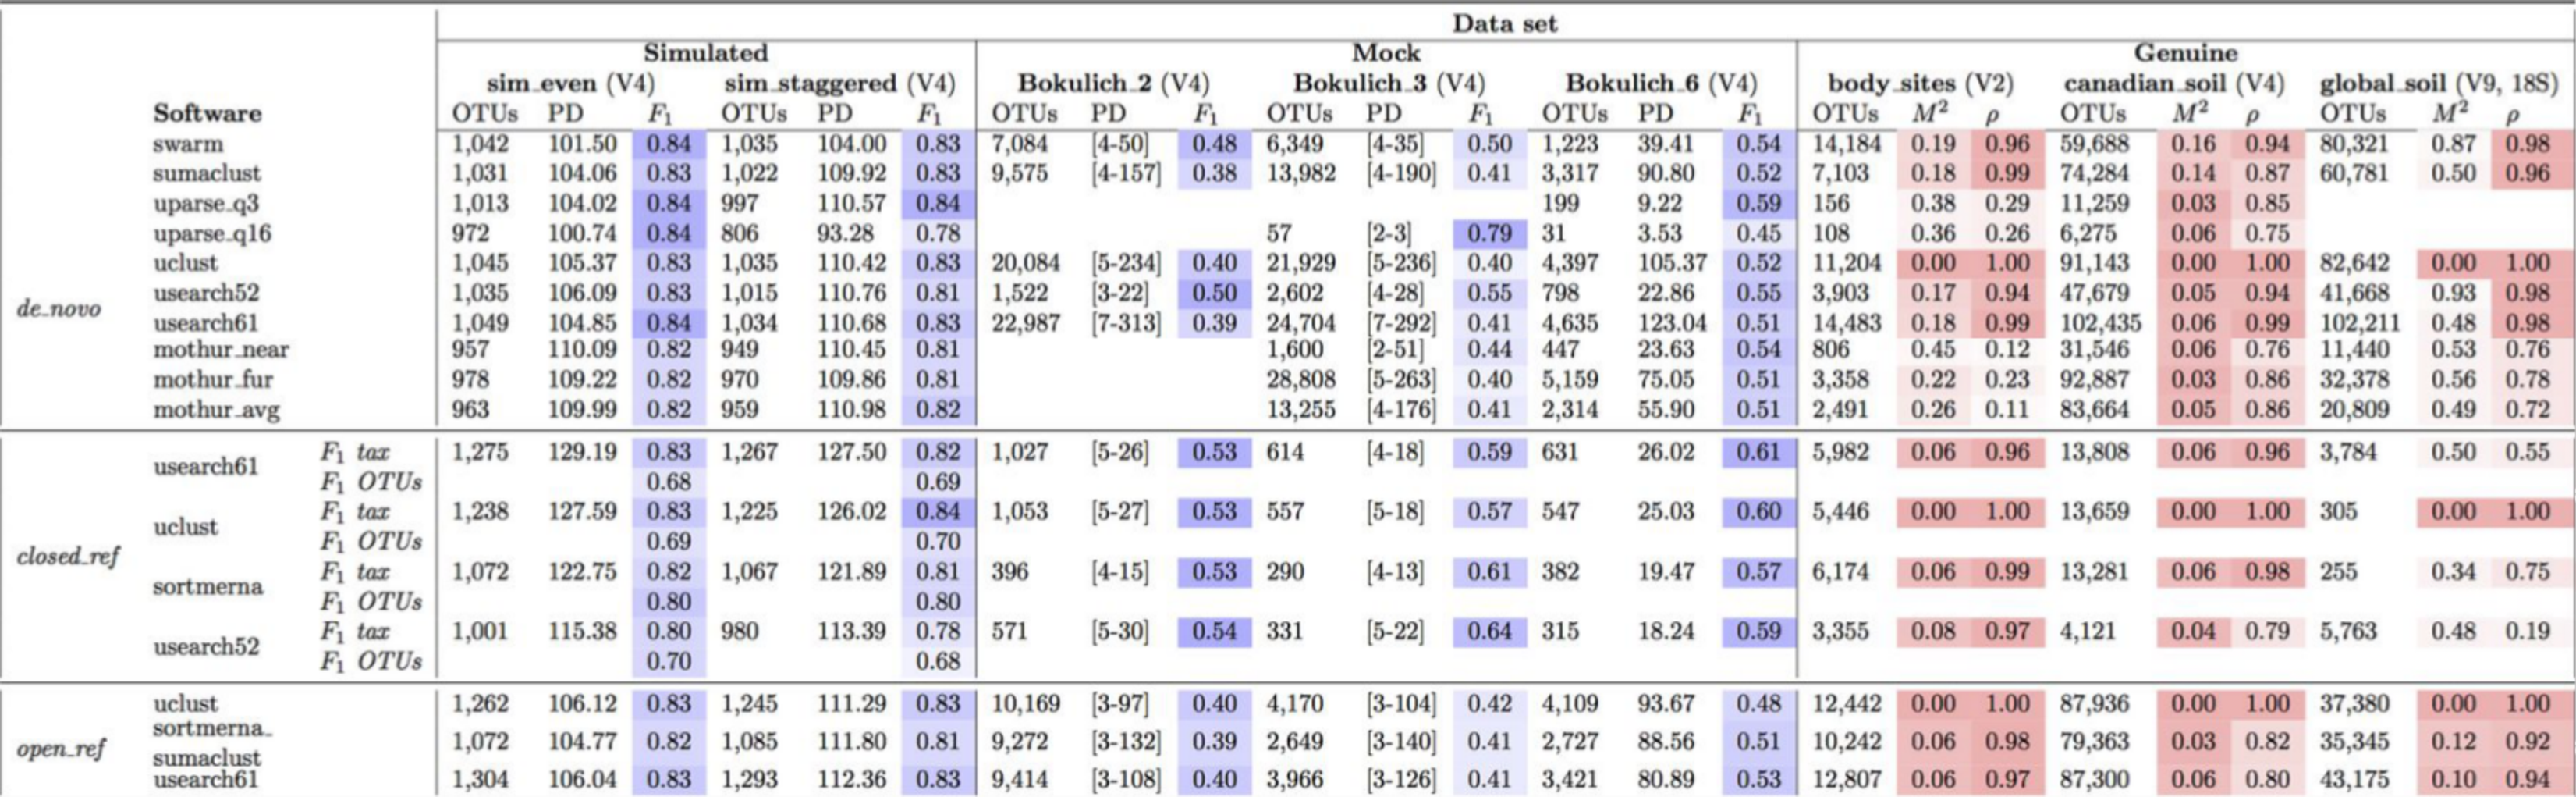
\includegraphics[width=\columnwidth]{chapter_otupicking_figures/stateArtT2.pdf}
\caption[Benchmark summary]{\textbf{Benchmark summary.} \gls{otu} counts do not
include singletons. F measure (F1) is for assigned taxonomies at the genus level.
The \gls{pd} whole-tree column for \emph{Bokulich\_2} and \emph{Bokulick\_3}
represent \gls{pd} intervals across various sampling depths. Procrustes $M^2$
(the sum of squared deviations or the dissimilarity of two datasets for UniFrac
\gls{pcoa}) and rho (Pearson's correlation coefficient for taxonomies at genus
level) values are with repect to UCLUST (default for \gls{qiime} versions 1.0.0
to 1.9.1). Monte Carlo $P$ values were not included, since all values were
$<0.05$ except for \emph{de novo} usearch52 versus uclust ($P = 0.09$). The darkest
blue shades represent the highest F1 scores, while the darkest red shades represent
results closest to those obtained with UCLUST}
\label{stateArtT2}
\end{figure}

We found that Swarm, SUMACLUST, UCLUST, and UPARSE (with relaxed parameters)
performed equally well on simulated datasets where the ground truth was well
established, with \emph{mothur\_average} and OTUCLUST closely behind. Despite
this controlled chimera-free environment, UPARSE with recommended parameters
reported the lowest accuracy for the \emph{sim\_staggered} data set, implying
that stringent quality filtering can cause a significant underestimation of
species abundance and diversity and lead to incorrect biological results. For
the mock communities, most tools were able to correctly detect the expected
number and identity of genera, but only UPARSE reported significantly fewer
false-positive taxa (followed by OTUCLUST and USEARCH). For UPARSE, this was
expected, as a large proportion of reads was filtered out prior to clustering,
leaving evidence of only the most abundant taxa (\gls{otu}s comprised of
hundreds of thousands of reads). The majority of false-positive taxa reported
by other tools were low-abundance \gls{otu}s that could be mapped to \gls{blast}’s NT
database with very high similarity ($E$ value, $<1e−50$). If the user’s primary
goal is to focus on the most abundant microbial profiles, low-abundance \gls{otu}s
may be filtered out postclustering, but care should be taken, as such low-abundance
\gls{otu}s can be important members of communities \cite{Shade2014}.

Although most open-source tools report an increased run time in comparison to UCLUST
and USEARCH ~\ref{stateArtF5}, they provide the benefit of finding significantly
fewer \gls{otu}s. In the case of SortMeRNA, longer reads (~150 \gls{bp}) are quicker
to align than the same number of shorter reads (~100 \gls{bp}) due to many fewer
high-scoring candidate reference sequences to analyze. Moreover, all of these tools
support multilevel multithreading and can easily scale to modern big-data processing
demands. An alternative to reducing run time is to filter out a substantial
number of reads, as done by UPARSE; unfortunately, the filtering parameters are
sensitive to different data, and choosing them manually by trial and error can be
a time-consuming task with unpredictable outcomes in diversity.

\begin{figure}[htbp]
\begin{center}
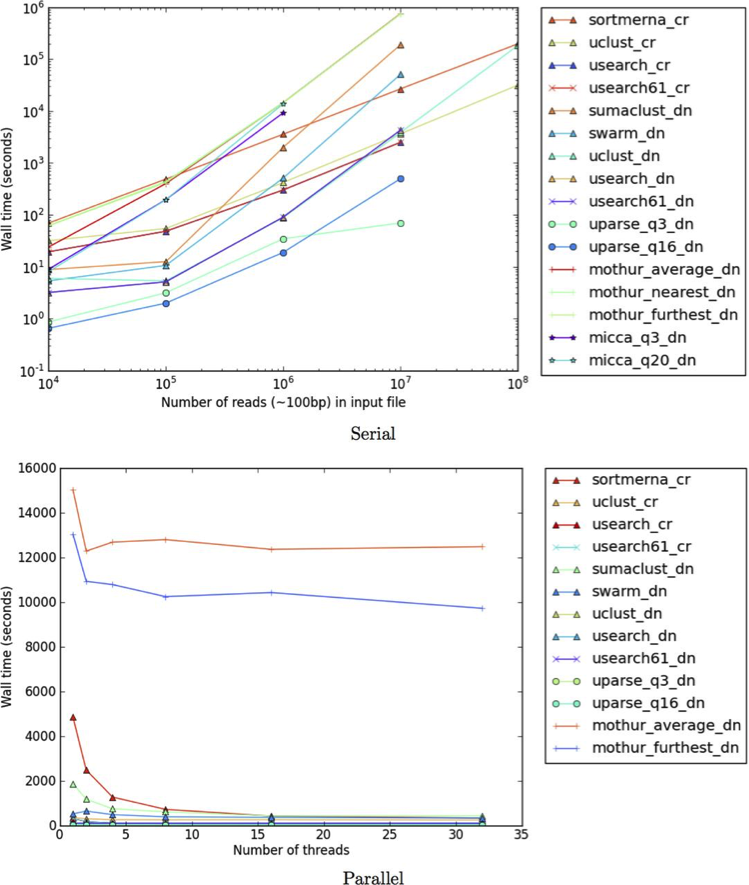
\includegraphics[height=0.55\textheight]{chapter_otupicking_figures/stateArtF5.png}
\end{center}
\caption[Runtime performance of all benchmarked software]{\textbf{Runtime performance of all benchmarked software.}
All tests were performed using 1 to 32 coers on Intel Xeon CPU E5-2640 v3 at 2.60 GHz.
Input files contained reads subsampled from the Global Gut \cite{Yatsunenko2012}.
For serial performance, some tools do not show results for $10^8$ reads due to
exceeding wall time limit (230 hours) or failed memory allocation. For parallel performance,
a single file containing 1 million Illumina sequences was used over multiple threads}
\label{stateArtF5}
\end{figure}

\subsection{Deblur rapidly resolves single-nucleotide community sequence patterns}\label{subsection_deblur}

Sections~\ref{subsection_openref} and~\ref{subsection_soa} were focused on
improving the performance of the \gls{otu} picking process for analyzing
microbial community datasets. \gls{otu}s are defined to approximate the species
richness of a sample, and reduce the effects of the sequencing error from \gls{ngs}
technologies. However, \gls{otu}s are based on an arbitrary sequence identity
threshold (typically 97\%) which reduces the phylogenetic resolution since two
sequences that are more similar than the identity threshold can't be differentiated.
To assess this problem, we presented a new method, Deblur, that instead of grouping
sequences based on an arbitrary sequence identy threshold, uses statistical
methods to find the underlying true sequence and remove erroneus sequences \cite{Amir2017}.

The following paragraphs have been adapted from the original publication in
\textsl{mSystems, 2016}. As a contributor of this manuscript, I was involved on
the discussions of the Deblur pipeline, I contributed to the source code, generated
figures for the manuscript and reviewed drafts of the manuscript.

Similar in concept to AmpliconNoise \cite{Quince2011}, a denoising method for
pyrosequencing, Deblur, like DADA2 \cite{Callahan2016} and UNOISE2 \cite{Edgar2016},
attempts to obtain single-nucleotide resolution from Illumina data with
statistical methods to infer the putative true sequences within a sample that
give rise to the distribution of observed error-prone sequences. Unlike DADA2 and
UNOISE2, Deblur operates on each sample independently. It compares
sequence-to-sequence Hamming distances within a sample to an upper-bound error
profile combined with a greedy algorithm to obtain single-nucleotide resolution.
The Deblur algorithm is implemented as follows (see Figure~\ref{figure_deblur}).
First, sequences are sorted by abundance. Second, from the most to least
abundant sequence, the number of predicted error-derived reads is subtracted
from neighboring reads based on their Hamming distance, using an upper bound on
the error probability. A parameterized maximal probability for indels
(defaulting to 0.01) and a parameterized mean read error rate for normalization
(defaulting to 0.5\%) are included. Finally, any sequence whose abundance drops
to 0 after a subtraction is removed from the list of valid sequences. Sequences
not considered to be valid (i.e., noise) are removed. After applying Deblur,
only reads likely to have been presented to the sequencer are retained.
However, it is possible that the reads would still contain chimeras originating
from PCR. Reads are filtered for de novo chimeras using UCHIME \cite{Edgar2011}
as implemented by VSEARCH \cite{Rognes2016} using modified parameters.

\begin{figure}[htbp]
\begin{center}
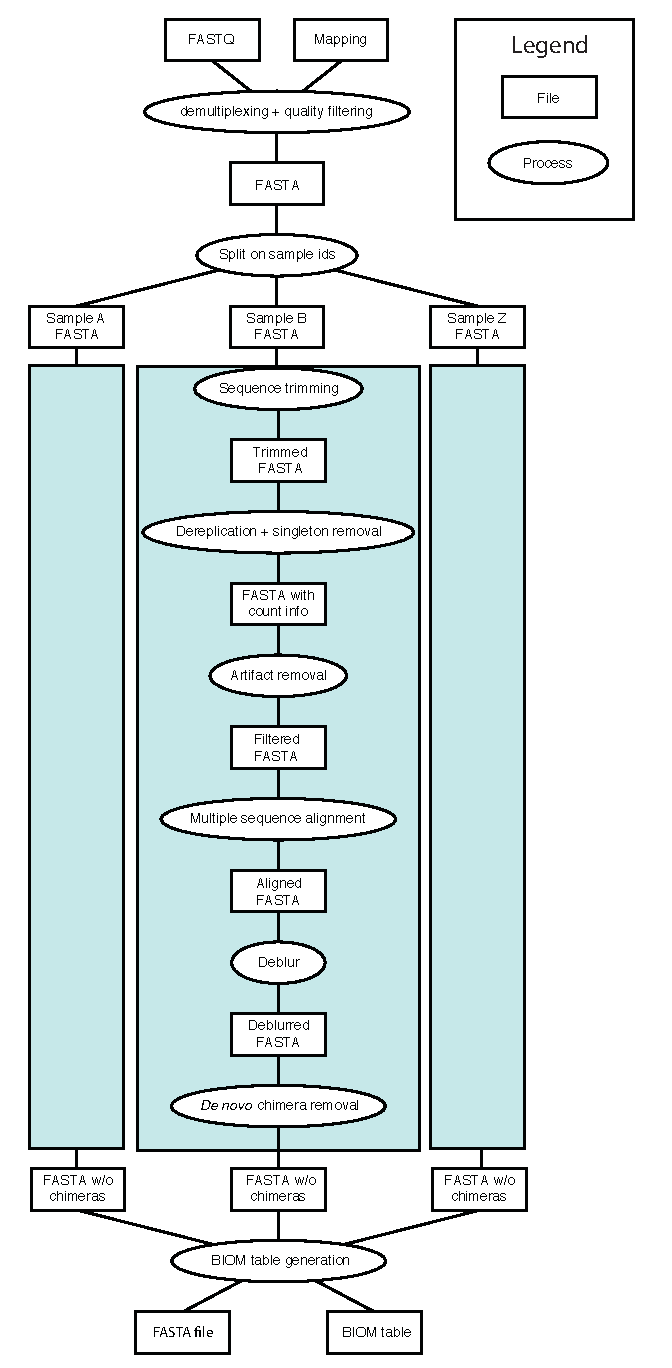
\includegraphics[height=0.70\textheight]{chapter_otupicking_figures/deblurWorkflow.pdf}
\end{center}
\caption[The deblur pipeline]{\textbf{The deblur pipeline.}
A demultiplexed and quality filtered fasta/fastq file (or a directory of per-sample
fasta/fastq files) is used as the input to the pipeline. Following initial
splitting to per-sample fasta files, all processing is done independently on each
sample. Sequences are trimmed and dereplicated with singletons removed. Reads are
then depleted from sequencing artifacts either using a set of known sequencing
artifacts (such as PhiX) (negative filtering) or using a set of known 16S sequences
(positive filtering). Resulting nonartifact reads are then aligned for easy indel
detection. This multiple sequence alignment is then used as the input for the Deblur
algorithm. Each Deblurred sample is then checked for de novo chimeras, and the
resulting s\gls{otu}s from all samples are combined into a single BIOM \cite{McDonald2012BIOM}
table (with sequences labeled as the s\gls{otu} IDs)}
\label{figure_deblur}
\end{figure}

Stability (i.e., obtaining the same s\gls{otu} across different samples) is becoming
critical as more study designs exploit existing samples from resources like the
Earth Microbiome Project \cite{Gilbert2014} or require integration of sequence
data collected over time such as the American Gut Project \footnote{\url{http://americangut.org}}.
We compared the levels of stability of Deblur and DADA2 using technical replicates
from a data set consisting of 40 individuals, each with one fecal sample sequenced
twice on two separate MiSeq runs \cite{Hildebrand2014}. s\gls{otu}s for each run were
assessed separately, and we compared the fractions of s\gls{otu}s from one run to
those present in the second run, as a function of the minimal s\gls{otu} frequency.
Deblur showed greater stability than DADA2 at a higher frequency cutoff (Figure ~\ref{figure_deblur_bench}-A),
indicating that a larger fraction of s\gls{otu}s from the first run were also identified in the second run.

Next, we compared DADA2 and Deblur using a complex natural community and a previously
published data set of fecal samples from two species of howler monkeys \cite{Amato2016}.
Deblur and DADA2 detected 1,938 and 1,636 s\gls{otu}s, respectively, after removal
of s\gls{otu}s with fewer than 10 total reads from each method. Following filtering,
about 70\% of the s\gls{otu}s were identical between the methods. As expected, both
methods identified differential s\gls{otu}s (permutation-based rank mean test;
0.1 false-discovery rate–Benjamini-Hochberg method [FDR-BH] control value) with 61\%
of Deblur s\gls{otu}s differentiating between primate species (1,193/1,938),
compared to 55\% of DADA2 s\gls{otu}s (891/1,636). To assess whether the
s\gls{otu}s unique to either method were from increased numbers of artifacts,
we used \gls{blast} \cite{Altschul1990} to compare each unique sequence against
nt/nr and plotted the fraction of s\gls{otu}s with zero, one, or two mismatches.
We observed that s\gls{otu}s unique to Deblur showed fewer mismatches than those
unique to DADA2 (Figure ~\ref{figure_deblur_bench}-B). The distribution of
s\gls{otu}s over the monkey samples suggests that the s\gls{otu}s unique to Deblur
are more plausible because they show a pattern similar to those identified by both
methods, whereas the s\gls{otu}s unique to DADA2 have markedly different patterns
of clusters of unique s\gls{otu}s within single samples (Figure ~\ref{figure_deblur_bench}-C).

Finally, to explore performance characteristics, we used a MiSeq run from the
stability analysis in order to assess computational space and time demands of DADA2,
Deblur, and UNOISE2 (where possible) over an increasing number of samples.
UNOISE2 was an order of magnitude faster than Deblur, while Deblur was an order of
magnitude faster than DADA2 (Figure ~\ref{figure_deblur_bench}-D).

\begin{figure}[htbp]
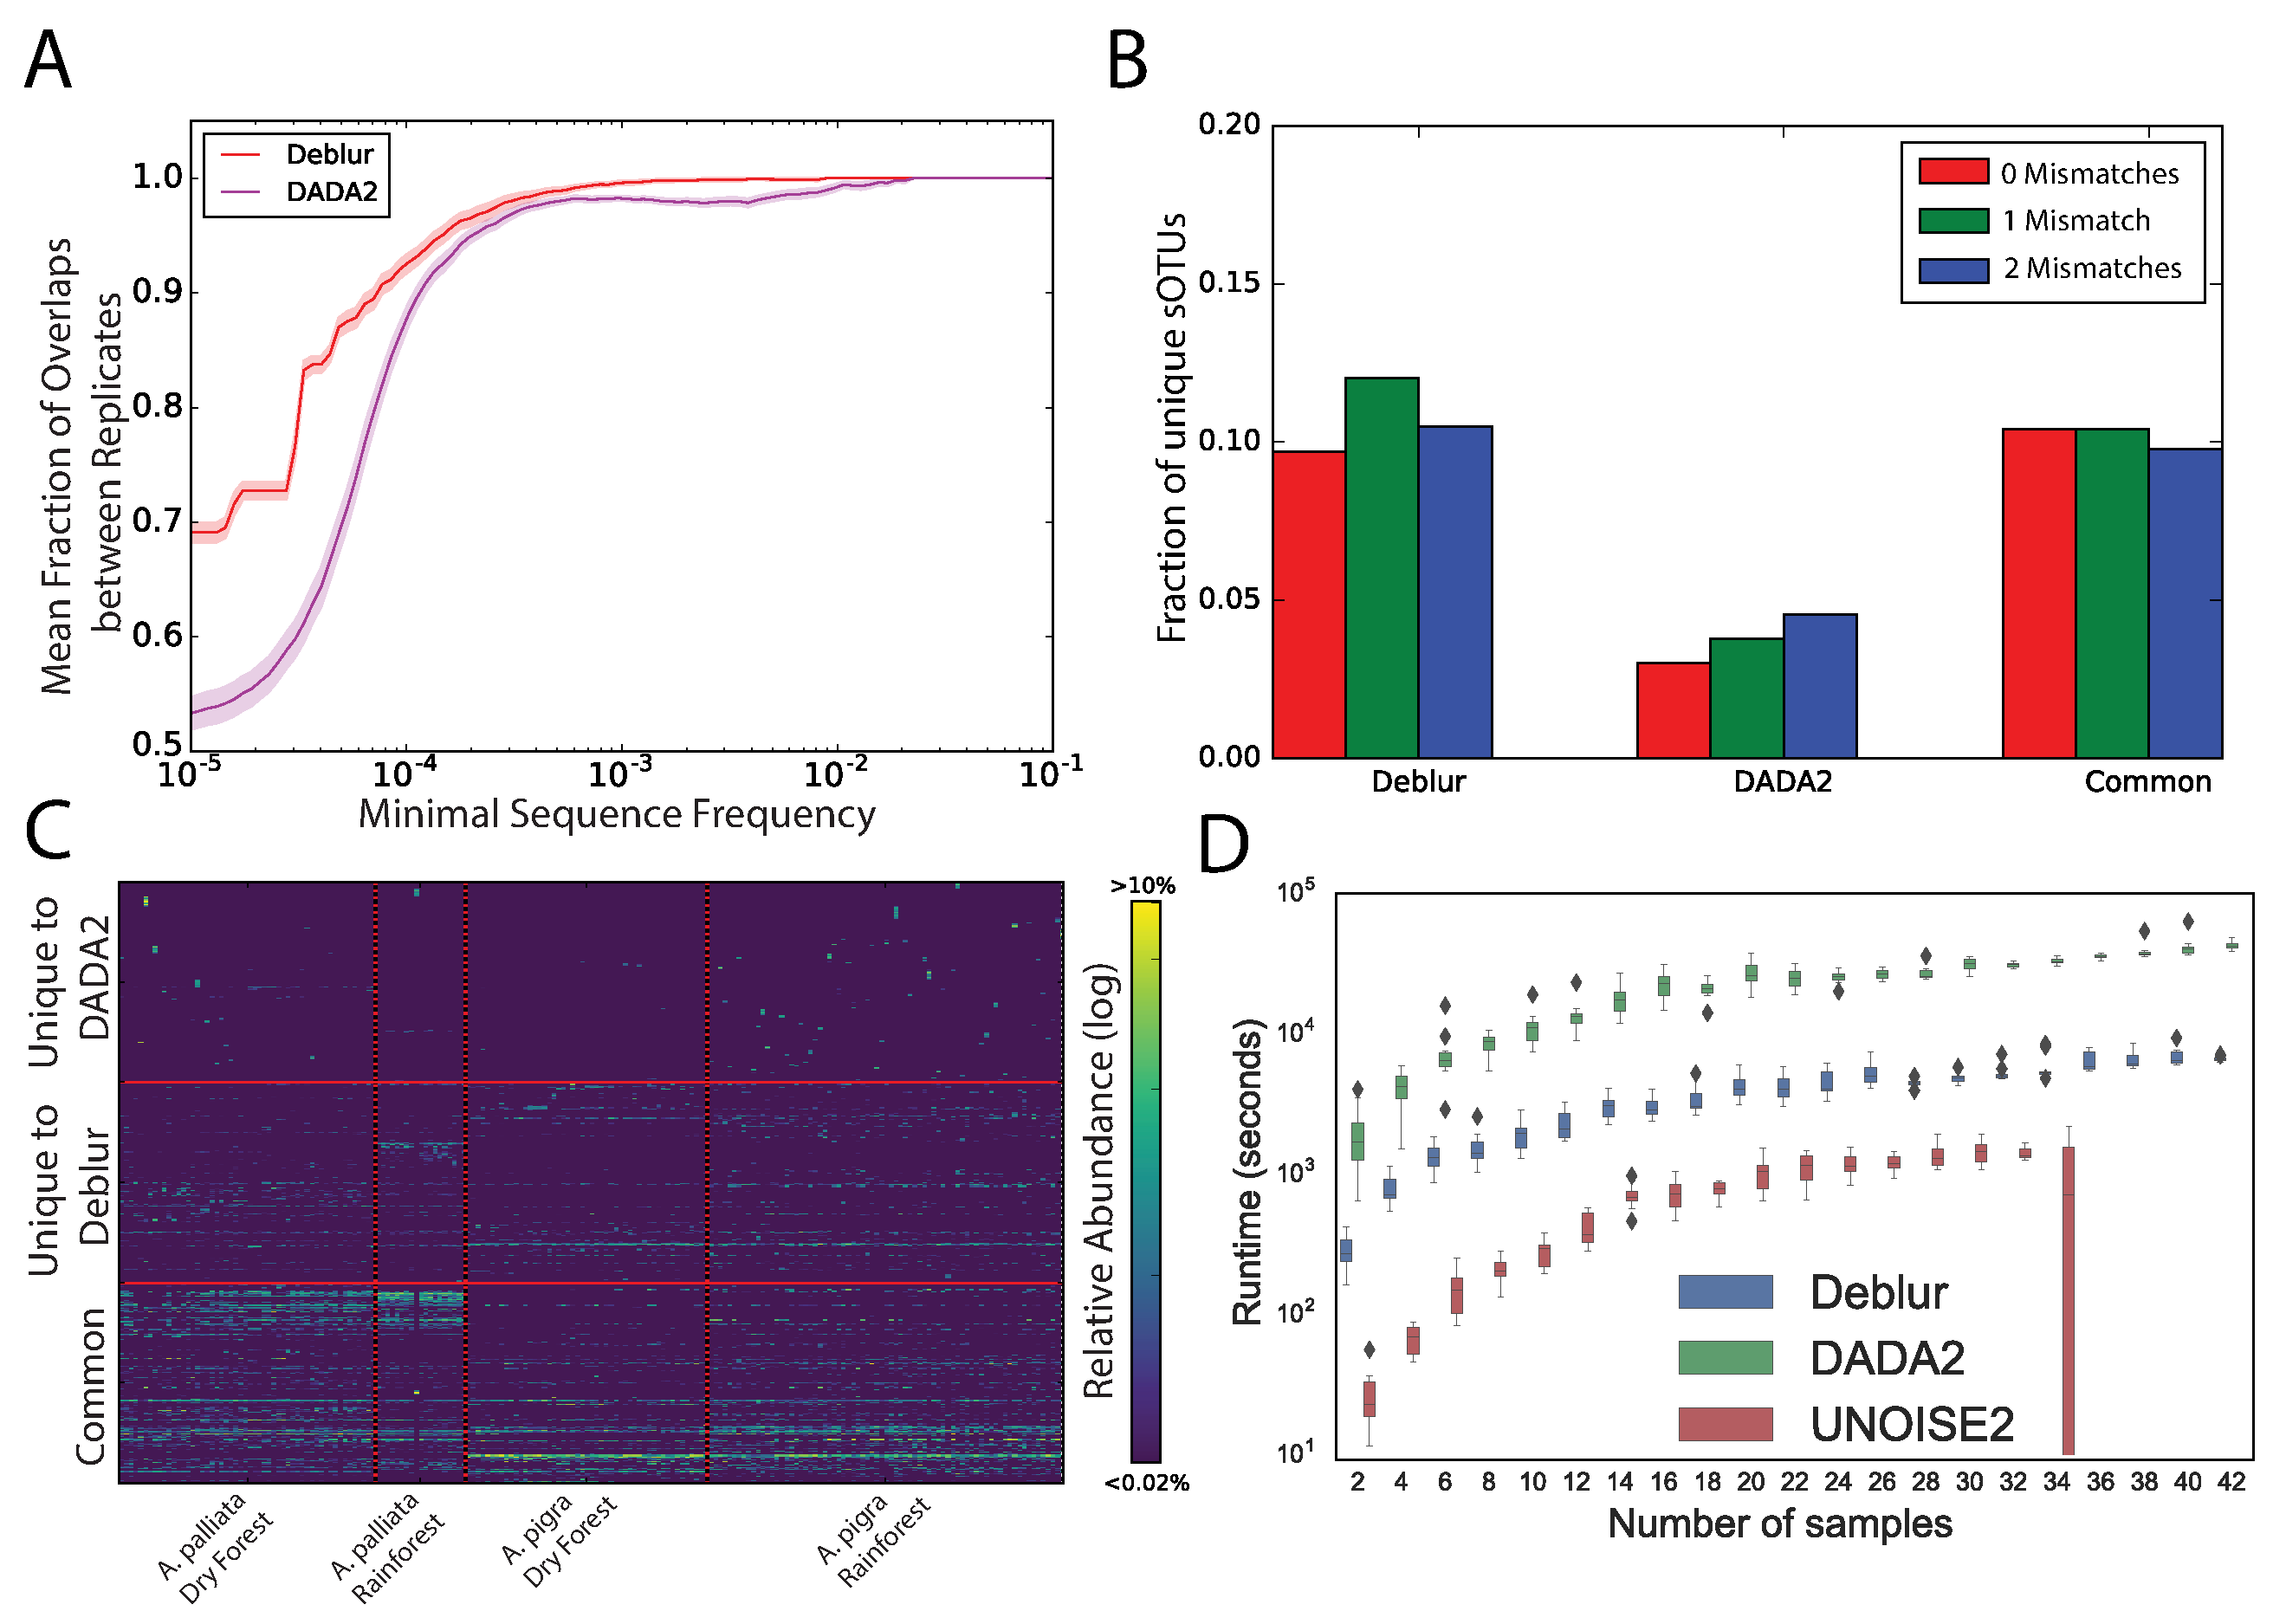
\includegraphics[width=\columnwidth]{chapter_otupicking_figures/deblurBench.pdf}
\caption[Benchmarks of \gls{otu} picking tools on natural communities]{\textbf{Benchmarks of \gls{otu} picking tools on natural communities.}
(A) Stability analysis on experimental technical repeats. Data indicate fractions
of overlapping s\gls{otu}s from two technical replicates in all \gls{otu}s as a
function of the minimal frequency threshold present in one of the repeats.
(B and C) Application of Deblur in the howler monkey data set. (B) Fraction of
sequences matching entries in the \gls{ncbi} nr/nt database
(as of 1 December 2016) with 0.1 or 2 mismatches (red, green, or blue, respectively)
from s\gls{otu}s unique to Deblur or to DADA2 or present in both (left to right).
(C) Heat maps showing s\gls{otu}s (rows) in common with Deblur and DADA2, as well
as those unique to Deblur and DADA2 (bottom, middle, and top rows, respectively).
Samples (columns) are sorted by species and habitat. A total of 200 s\gls{otu}s per group
(i.e., common, unique to Deblur, or unique to DADA2) were randomly selected for
visualization purposes. (D) Single-threaded runtime comparison of Deblur, DADA2,
and UNOISE2 against one of the stability MiSeq runs at increasing numbers of samples.}
\label{figure_deblur_bench}
\end{figure}
